\documentclass{article}
\usepackage{graphicx}
\usepackage{amsmath}
\usepackage{polski}
\usepackage[utf8]{inputenc}
\title{UOA ćwiczenie 3}
\author{Denis Firat}
\date{June 2020}

\begin{document}

\maketitle

\section{Cel ćwiczenia}
Celem ćwiczenia jest zapoznanie się z przekaźnikami, stycznikami, urządzeniami wykonawczymi , Falownikami i programem Logo.

\section{Odpowiedzi na punkt 1}
\subsection{Układ start-stop}
\begin{figure}[!ht]
    \centering
    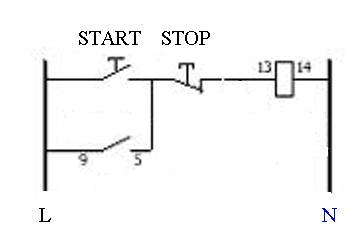
\includegraphics[scale=0.8]{startstop.jpg}
    \caption{Prosty schemat układu START-STOP w języku ladder}
\end{figure}
Układ start-stop jest jednym z prostszych układów, które zapewniają
podtrzymanie sygnału. Załączenie przycisku start, zastila cewkę przekaźnika.
równolegle do przycisku start podłączony jest jeden z zacisków przekaźnika. To
właśnie ten zacisk zapewnia podtrzymanie, dopiero naciśnięcie stop, odcina dopływ prądu do
cewki i zwalnia podtrzymanie.
\subsection{Różnica między stycznikiem, a przekaźnikiem}
Styczniki używane są w obwodach wysoko prądowych(np. wykonawczych), a przekaźniki
używane są w obwodach niskoprądowych(np. sterowniczych). Z tego powodu różnią się rozmiarem oraz
obciążalnością styków.
\subsection{Przekaźniki elektroniczne}\documentclass{article}
\usepackage{graphicx}
\usepackage{amsmath}
\usepackage{polski}
\usepackage[utf8]{inputenc}
\title{UOA ćwiczenie 3}
\author{Denis Firat}
\date{June 2020}

\begin{document}

\maketitle

\section{Cel ćwiczenia}
Celem ćwiczenia jest zapoznanie się z przekaźnikami, stycznikami, urządzeniami wykonawczymi , Falownikami i programem Logo.

\section{Odpowiedzi na punkt 1}
\subsection{Układ start-stop}
\begin{figure}[!ht]
    \centering
    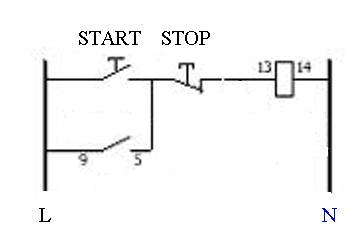
\includegraphics[scale=0.8]{startstop.jpg}
    \caption{Prosty schemat układu START-STOP w języku ladder}
\end{figure}
Układ start-stop jest jednym z prostszych układów, które zapewniają
podtrzymanie sygnału. Załączenie przycisku start, zastila cewkę przekaźnika.
równolegle do przycisku start podłączony jest jeden z zacisków przekaźnika. To
właśnie ten zacisk zapewnia podtrzymanie, dopiero naciśnięcie stop, odcina dopływ prądu do
cewki i zwalnia podtrzymanie.
\subsection{Różnica między stycznikiem, a przekaźnikiem}
Styczniki używane są w obwodach wysoko prądowych(np. wykonawczych), a przekaźniki
używane są w obwodach niskoprądowych(np. sterowniczych). Z tego powodu różnią się rozmiarem oraz
obciążalnością styków.
\subsection{Przekaźniki elektroniczne}
Przekaźniki elektroniczne, są to układy elektroniczne zapewniające działanie
zbliżone do przekaźników elektrycznych. Cechują się cichą pracą, brakiem iskrzenia i dłuższą żywotnością.
\subsection{Przekaźniki prądu zmiennego, a stałego}
Przekaźniki prądu zmiennego zawierają w sobie dodatkowy zwart zwój, prąd w tym zwartym zwoju przesunięty w fazie o 90 stopni,
względem prądu cewki. Dzięki temu, nawet gdy prąd cewki przekracza 0V (bez dodatkowego zwartego zwoju, w tym momencie przekaźnik by się rozwarł)
to zwarcie jest podtrzymywane przez dodatkowy zwarty zwój.
\section{Praca w programie Logo}
Układ start-stop wykonałem z pomocą przerzutnika RS. Start podłączony jest do złącza set, a stop do złącza reset. Jako wejścia dałem dwa przyciski. Po przetestowaniu, program działał zgodnie z zasadą działania układów start-stop. Gdy dodałem do układu przerzutnik asynchroniczny, udało mi się wykonać układ z drugiego podpunktu.
\begin{figure}[!h]
    \centering
    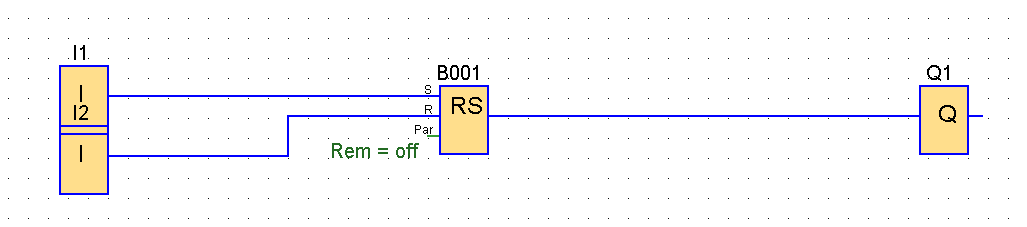
\includegraphics[scale=0.5]{startstoplogo.png}
    \caption{Układ start-stop w Logo}
    \label{fig:my_label}
\end{figure}
\begin{figure}[!h]
    \centering
    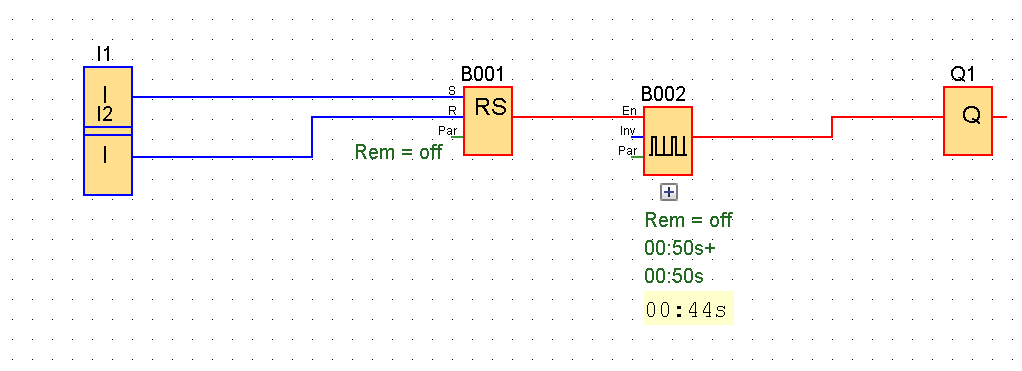
\includegraphics[scale=0.5]{STARTSTOPHZ.png}
    \caption{Układ start-stop z wyjściem przełączającym się z f=-0,5 Hz}
    \label{fig:my_label}
\end{figure}
\section{Przetwornica częstotliwości}
\begin{itemize}
    \item Falownik tourządzenie elektryczne zamieniające prąd stały (ang. direct current, DC), którym jest zasilane, na prąd przemienny (ang. alternating current, AC) o regulowanej częstotliwości wyjściowej.
    \item Falowniki służą do zasilania silników elektrycznych asynchronicznych
    \item Możliwe połączenie to gwiazda lub trójkąt.
    \item nie, stosując falownik zasilany 1-fazowo możemy użyć tylko połącznia w gwiazdę
\end{itemize}
\end{document}

Przekaźniki elektroniczne, są to układy elektroniczne zapewniające działanie
zbliżone do przekaźników elektrycznych. Cechują się cichą pracą, brakiem iskrzenia i dłuższą żywotnością.
\subsection{Przekaźniki prądu zmiennego, a stałego}
Przekaźniki prądu zmiennego zawierają w sobie dodatkowy zwart zwój, prąd w tym zwartym zwoju przesunięty w fazie o 90 stopni,
względem prądu cewki. Dzięki temu, nawet gdy prąd cewki przekracza 0V (bez dodatkowego zwartego zwoju, w tym momencie przekaźnik by się rozwarł)
to zwarcie jest podtrzymywane przez dodatkowy zwarty zwój.
\subsection{Oznaczenia na schematach}
\end{document}
